\chapter*{Appendices}
\addcontentsline{toc}{chapter}{Appendices}
\thispagestyle{MyStyle}

\begin{figure}[H]
  \centering
  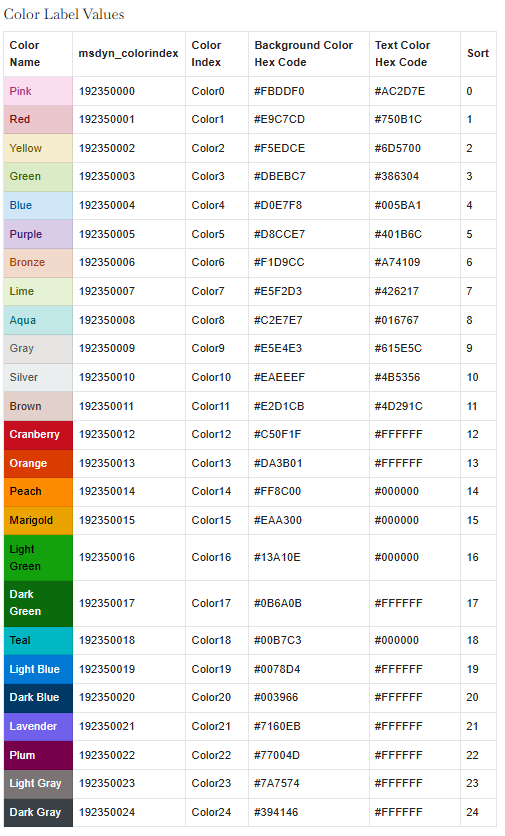
\includegraphics[width=0.62\textwidth,max width=\textwidth]{images/image71.png}
  \caption{image71}
  \label{fig:image71}
\end{figure}

\url{https://christine-payton.com/microsoft-planner-project-for-the-web-color-label-values/}

\begin{figure}[H]
  \centering
  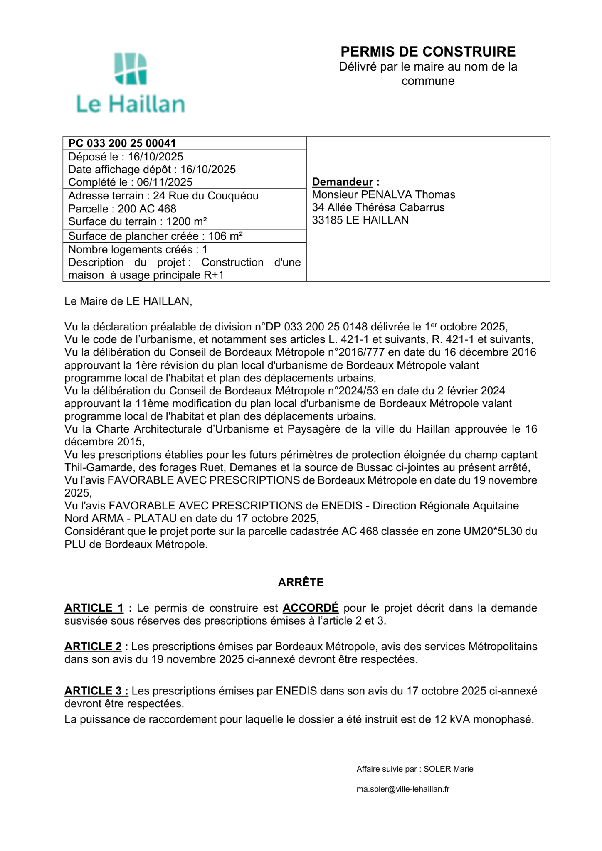
\includegraphics[width=0.62\textwidth,max width=\textwidth]{images/image72.png}
  \caption{image72}
  \label{fig:image72}
\end{figure}

\begin{figure}[H]
  \centering
  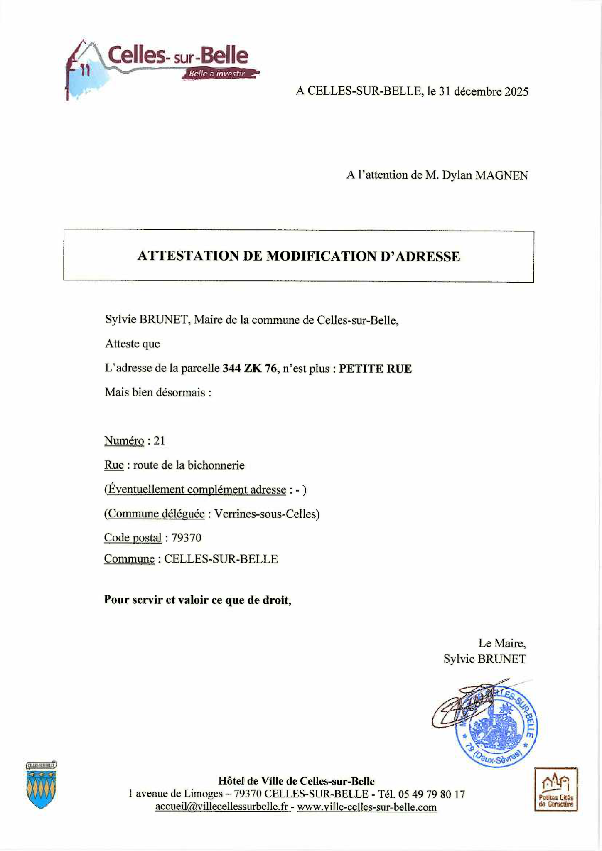
\includegraphics[width=0.62\textwidth,max width=\textwidth]{images/image73.png}
  \caption{image73}
  \label{fig:image73}
\end{figure}

\begin{figure}[H]
  \centering
  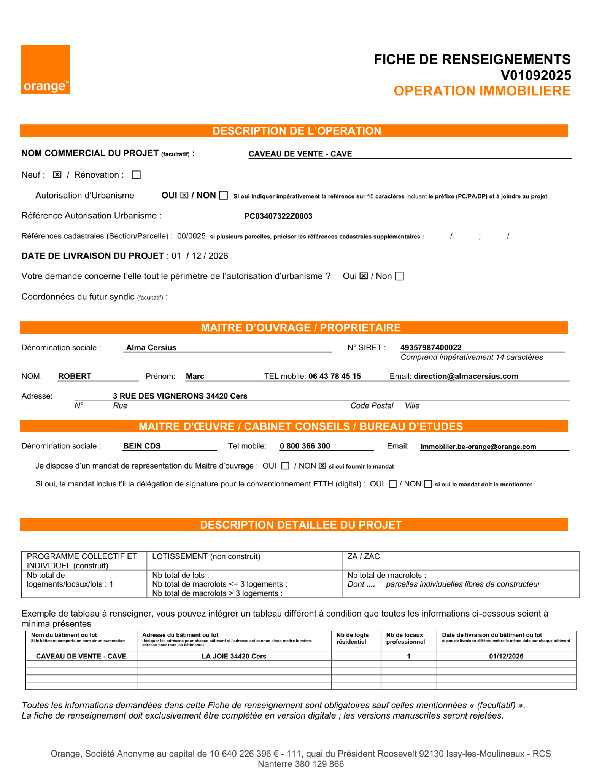
\includegraphics[width=0.62\textwidth,max width=\textwidth]{images/image74.png}
  \caption{image74}
  \label{fig:image74}
\end{figure}

\begin{figure}[H]
  \centering
  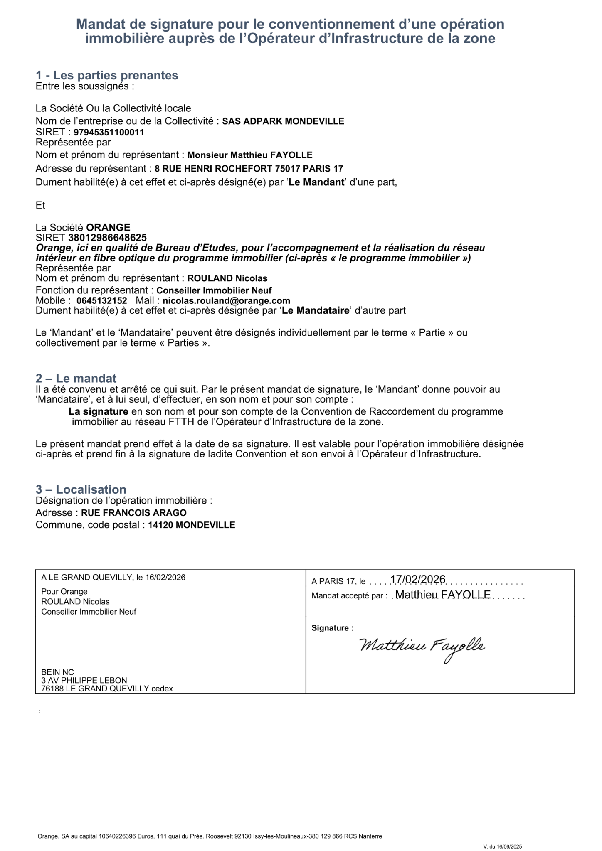
\includegraphics[width=0.62\textwidth,max width=\textwidth]{images/image75.png}
  \caption{image75}
  \label{fig:image75}
\end{figure}

\begin{figure}[H]
  \centering
  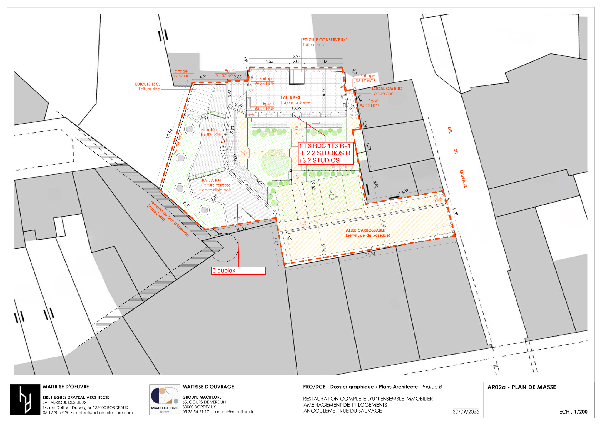
\includegraphics[width=0.62\textwidth,max width=\textwidth]{images/image76.png}
  \caption{image76}
  \label{fig:image76}
\end{figure}

\begin{figure}[H]
  \centering
  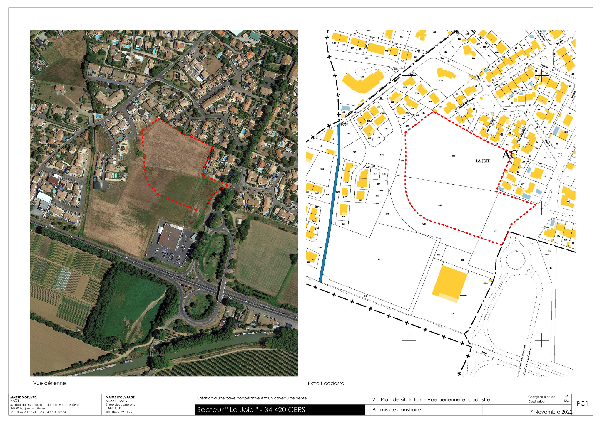
\includegraphics[width=0.62\textwidth,max width=\textwidth]{images/image77.png}
  \caption{image77}
  \label{fig:image77}
\end{figure}
